%%%%%%%%%%%%%%%%%%%%%%%%%%%%%%%%%%%%%%%%%%%%%%%%%%%%%%%%%%%%%%%%%%%%%%%%%%%%%%%%
%
%   Semester project, fall term 2014
%   Author: Jakob Ehrl, born 01/24/91
%   Study program: Computer science, MA 1
%   
%   Professor Dr. Francesco Mondada
%   Assistant: Dr. Stefan Witwicki
%
%%%%%%%%%%%%%%%%%%%%%%%%%%%%%%%%%%%%%%%%%%%%%%%%%%%%%%%%%%%%%%%%%%%%%%%%%%%%%%%%%

\chapter{Schematics and Implementation}

In this section is described the connection between the different modules, voltage sources, and the signal cables.

\section{Modules connection}

The main modules are connected together, with a central processing brain, the Odroid-C1.

\begin{figure}[H]
  \centering
  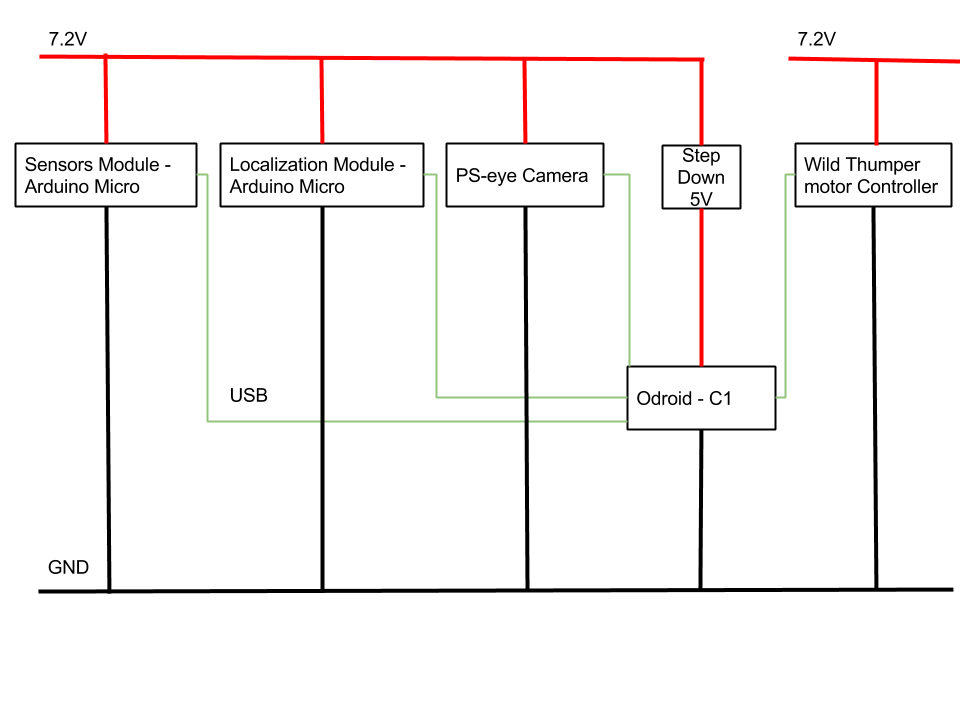
\includegraphics[width=0.8\textwidth]{GlobalConnection.png}
  \caption{The Global abstract connection between the different modules.}
\label{fig:GlobalConnection}
\end{figure}

In the Figure \ref{fig:GlobalConnection} above, is represented the connection diagram between the main modules. As it can be observed, the communication connections between these modules are all USB ( green wire) . This will reduce the number of cables, and ease the communication, as it is an asynchronous protocol, which is widely used and very documented for the arduinos and odroid.\\

Everything is supplied by two battery packs of 7.2 Volts, but have a common ground. The reason for decoupling the wild thumper power supply from the rest comes from the high demand in current required for the motors. This current flow can (if higher than the 10 A of the fuse) burn the fuse for in the power rack. Another reason is that the motors draw much current (2.2 Amps per motor at stall) and if the odroid is connected to the same battery it can happen that the current instability will cause the odroid to fail.

The odroid is connected to a step down voltage regulator, because it needs a stable 5 volts power supply to function correctly.

\section{Sensor Module}

The sensors module, as described in it's respective section, is connected to all the range sensors in the robot. It can also control the brush motor and the Dynamixel smart Servo. An other feature is to read the current that is flowing through the brush motor.

\begin{figure}[H]
  \centering
  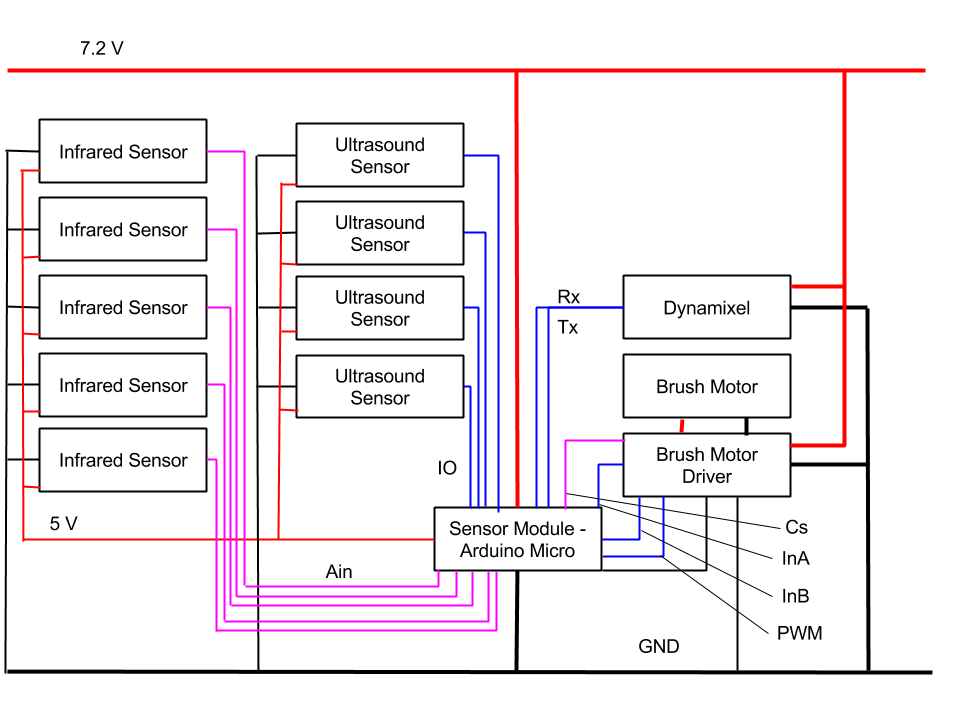
\includegraphics[width=0.8\textwidth]{Arduino1Connection.png}
  \caption{The Sensors module, and it's connections.}
\label{fig:ard1connection}
\end{figure}

As it can be seen in Figure \ref{fig:ard1connection} above, the sensors module is connected to many different sensors. With 20 IO pins and 7 Analog input pins, the arduino Micro is also powerful enough to read, interpred, and connect to all those sensors. In purple are all the analog wires, and blue the IO pins. The Cs is a special pin on the motor driver that allows to read the current flowing through the motor. Each 140mV read on this pin corresponds to 1 Amp on the motor. For the dynamixel, as described earlier, the two serial wires are connected together with a resistance in between to simulate a half duplex connection. The ultrasound sensors, as well have both echo and ping pins connected together with a resistance in between, in order to reduce the number of pins used on the arduino micro, and facilitate the connections.\\

%\textbf{From the datasheets, the IR sensors draw 30mA and the Ultrasound Sensors draw 15mA. As a total, only the sensors draw 210 mA. From tests done with the arduino micro, the 5Volts output pin cannot supply such high demands in current. As a solution, it is also possible to conenct some sensors power supply to the wild thumper. RISKY}\\

The three other IO pins connected to the motor driver are just controls for the motor. The motor driver needs two power supplies. One is for the input logic, 5V, and the other is for the motor output (we used the battery 7.2 V power supply).

\section{Localization Module}

The localization module is, as described in the section previously, the module that uses 6 line sensor arrays and a compass to locate the position and yaw of the robot. 

\begin{figure}[H]
  \centering
  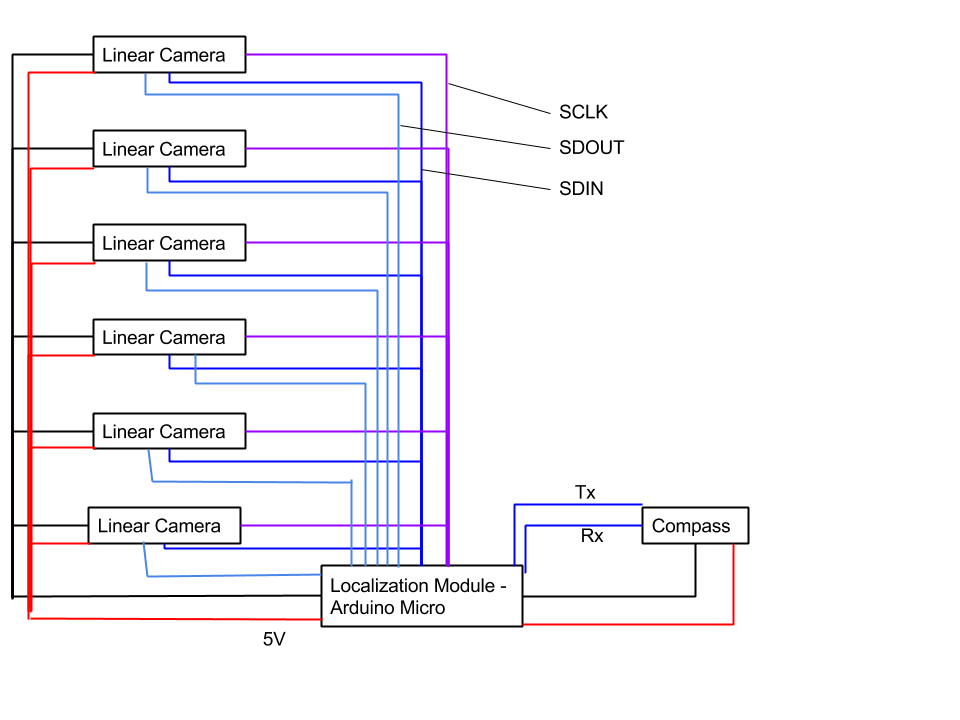
\includegraphics[width=0.8\textwidth]{Arduino2Connection.png}
  \caption{The Localization module, and it's connections.}
\label{fig:ard2connection}
\end{figure}

The connection between the arduino micro and the sensors is shown in the Figure \ref{fig:ard2connection} above. The compass uses a simple serial connection, and the arduino micro has two of them ( USB and serial pins). For the linear cameras, three lines were necessary. SCLK, the clock, can be common between the sensors, since it does not have any effect if no data is transmitted. %The SDIN lines are soldered together as well, XXXXXXXXXXXXXXXXXXXXXXXXXXXXXXXXXXXXXXXX
%XXXXXXXXXXXXXXXXXXXXXXXXXXXXXXXXXXXXXXXXXXX
%XXXXXXXXXXXXXXXXXXXXXXXXXXXXXXXx
%XXXXXXXXXXXXXXXXXXXXXXXXXXXXXXX
%XXXXXXXXXXXXXXXXXXXXXXXXXXXXXXX

\section{Motor driver module}

The motor driver module has very simple connections. The only devices it is controlling are the motors, and the tailgate servo.

\begin{figure}[H]
  \centering
  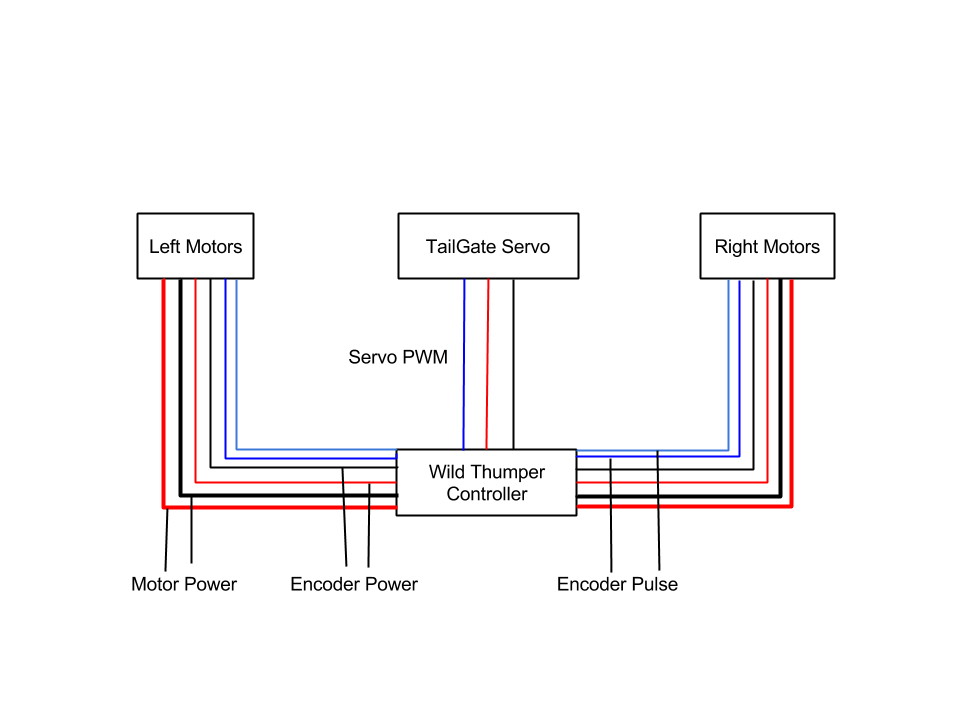
\includegraphics[width=0.8\textwidth]{WildThumperConnection.png}
  \caption{The Motor Driver Module, and it's connections.}
\label{fig:wtconnection}
\end{figure}

Seen in Figure \ref{fig:wtconnection} above is the connection diagram of the wild thumper motor controller. The only signals it is reading are the motor encoders, which allow to estimate a precise speed, and position of the wheels.

%\chapter{Implementation}
%how everything was connected, connectors etc.. battery... 

\chapter{Results}
%how the robot worked

\chapter{Conclusion}
%duh

\chapter{Annex}

\begin{figure}[H]
  \centering
  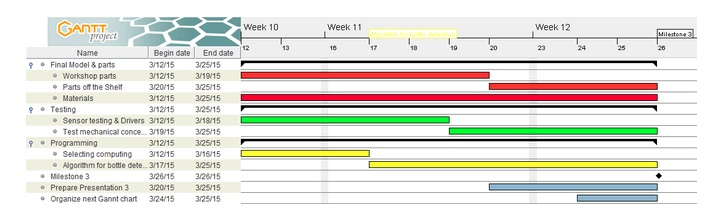
\includegraphics[width=0.8\textwidth]{GanttChart1.jpg}
  \caption{Gannt Chart until the third milestone.}
\label{fig:gannt1}
\end{figure}

\begin{figure}[H]
  \centering
  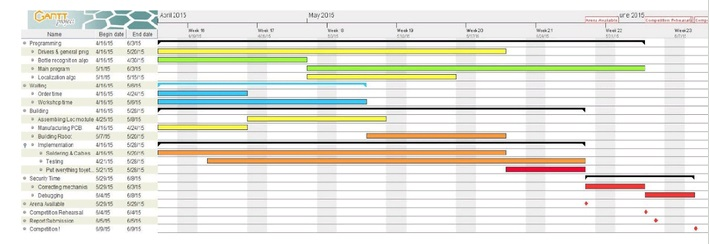
\includegraphics[width=0.8\textwidth]{GanttChart2.jpg}
  \caption{Gannt Chart until the end of the competition.}
\label{fig:gannt2}
\end{figure}